\documentclass[12pt, letterpaper, twoside]{article}
\usepackage[utf8]{inputenc}
\usepackage{graphicx}
\usepackage{amsmath}
\usepackage{parskip}
\usepackage{geometry}
\graphicspath{{images/}}

\title{My \LaTeX{} Learning Road, From Zero to Inf}
\author{Guanzheng Wang, Northwesten Polytechnical }
\date{November 1, 2020}

\geometry{left=2.0cm,right=2.0cm,top=3.0cm,bottom=3.0cm}
\begin{document}
% We are going to write a comments, which will not be printed to the pdf file
\maketitle

\tableofcontents 

\newpage
\begin{abstract}
This paper is something when practicing LateX, and this is just an abstract. Let's begin from now on, come to use LaTeX more and more.
\end{abstract}


\newpage

\part{Beginnings}

\section{Let We Go}


First document. Now we are going to change our line to a new one.\\
Let's use another ways.
\newline
In the past few years, I have learned LaTex for many times, but I have not wrote even a real article. This make me still feel unfamiliar with LaTex.



% bold, italics and underlining
Some of the \textbf{greatest} discoveries in \underline{science} were made by \textbf{\textit{accident}}.

% emph
Some of the greatest \emph{discoveries} in science were mde by accident.

\textit{Some of the greatest \emph{discoveries} in science were made by accident.}

\textbf{Some of the greatest \emph{discoveries} in science were made by accident.}


% add a picture
\begin{figure}[h]
	\centering
	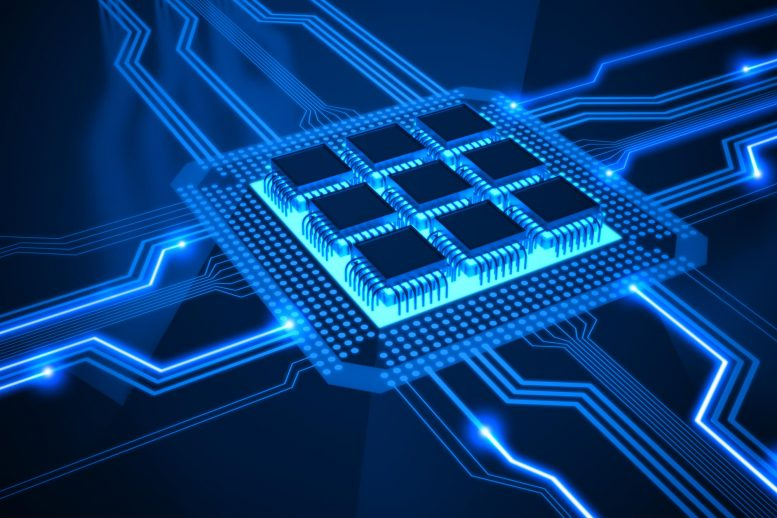
\includegraphics[width=0.5\textwidth]{parallel_computing}
	\caption{a fig of processor}
	\label{fig:processor}
\end{figure}

As you can see in the Figure \ref{fig:processor}. Also in the page \pageref{fig:processor} is the same example.


So what about the other things?
% add a list
\begin{itemize}
	\item CPU: I9-9900KF
	\item GPU: RTX-2080
	\item RAM: 32GB DDR4
\end{itemize}


There are many great computers for game users or professors. I used to like God of War, child brand of Hasee, but now I tend to but clevo machines directly.
% add an ordered list
\begin{enumerate}
	\item Clevo P870
	\item Clevo P775
\end{enumerate}



\section{Phisics}


In Physics, the mass-energy equivalence is stated by the equation $E=mc^2$, discovered in 1905 by Albert Einstein.

We can print it via other methods:
\[ E=mc^2 \], or:
\begin{equation}
E=mc^2
\end{equation}


Let's see something different.\\
Subscripts in math mode are written as $a_b$ and superscripts are written as $a^b$. These can be combined an nested to write expressions such as 
\begin{equation}
T^{i_1 i_2 \dots i_p}_{j_1 j_2 \dots j_q} = T(x^{i_1}, \dots, x^{i_p}, e_{j_1}, \dots, e_{j_q})
\end{equation}

We write integrals using $\int$ and fractions using $\frac{a}{b}$. Limits are placed on integrals using superscripts and  subscripts:

\begin{equation}
\int_0^1 \frac{dx}{e^x}=\frac{e-1}{e}
\end{equation}

Lower case Greek letters are written as $\omega$ $\delta$ etc. while upper case Greek letters are written as $\Omega$ $\Delta$.

Mathematical operations are prefixed with a backslash as $\sin(\beta)$, $\cos(\alpha)$, $\log(x)$ etc.



\part{Go on the next part}

\section{Draw a table}


Let's do something special.

Next, we are going to creat a table.
\begin{center}
	\begin{tabular}{|c|r|c|}
		\hline
		cell1 & cell2 & cell3 \\
		\hline		
		cell4 & cell5 & cell6 \\
		\hline		
		cell7 & cell8 & cell9 \\
		\hline
	\end{tabular}
\end{center}

\section{Do something more complex}
Let's see another example:\\
Table \ref{table:Just an example} is an example of referenced \LaTeX{} elements.
\begin{table}[h!]
	\begin{center}
		\begin{tabular}{||c c c c||}
		\hline
		Col1 & Col2 & Col3 & Col4 \\ [0.5ex]
		\hline\hline
		1 & 6 & 87837 & 787 \\
		\hline
		2 & 7 & 78 & 5417 \\ [1ex]
		\hline	
		\end{tabular}
		\caption{Table to test captions and labels}
		\label{table:Just an example}
	\end{center}
\end{table}



\end{document}